\begin{figure}[h]
      \centering   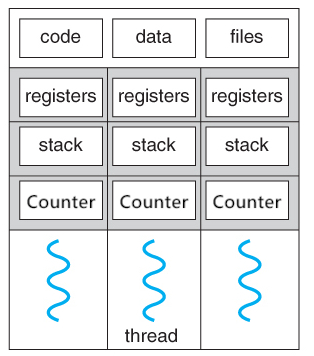
\includegraphics[scale=2]{./images/threads_01.jpeg}
\end{figure}

\begin{enumerate}
    \item zzz
    \item zzz
    \item zzz
    \item zzz
\end{enumerate}

\begin{minipage}{\linewidth}     \end{minipage}


\begin{myTableStyle} \begin{tabular}{ |m{2cm}|m{3cm}|m{4cm}|m{2cm}| } \hline
    Binary Tree & \makecell[l]{ A\\ B }  &  zzz &  zzz  \\ \hline
\end{tabular} \end{myTableStyle} \vspace{0.08in}


\lstinputlisting[language=C, firstline=2, lastline=20]{tree_programs_code.c}

\begin{lstlisting}  \end{lstlisting}

\lstinputlisting[language=Octave]{BitXorMatrix.m}

\begin{myTree}
  \node [squarednode,draw] [red] (node_a){root}
    child
    {
        node [circle,draw] (node_b) {b}
        child
        {
            node [circle,draw] (node_e) {e}
        }
        child
        {
            node [circle,draw] (node_f) {f}
        }
    }
    child
    {
        node [circle,draw] (node_d){d}
        child
        {
            node [circle,draw] (node_g) {g}
        }
        child
        {
            node [circle,draw] (node_h) {h}
        }
    };
\end{myTree}


\Theta  \omega  \Omega  \log_{a}b


\begin{comment}

\begin{questyle}
  \question  zzz  (GATE-zzz)

  \begin{choices}
    \choice         zzz
    \choice         zzz
    \choice         zzz
    \choice         zzz
    \CorrectChoice
  \end{choices}
\end{questyle}

    oneparchoices     \fillin[]

\end{comment}

